\documentclass[12pt]{article}


\usepackage[utf8]{inputenc}
\usepackage[a4paper,top=3cm,bottom=2cm,left=3cm,right=3cm,marginparwidth=1.75cm]{geometry}
\usepackage[nodayofweek]{datetime}
\usepackage{tabularx}
\usepackage[small]{titlesec}
\usepackage{graphicx}
\usepackage{tabularx}
\usepackage{amsmath}
\usepackage{fancyvrb}
\newcolumntype{L}[1]{>{\raggedright\arraybackslash}p{#1}}
\newcolumntype{C}[1]{>{\centering\arraybackslash}p{#1}}
\newcolumntype{R}[1]{>{\raggedleft\arraybackslash}p{#1}}

\begin{document}

\begin{titlepage}
    \begin{center}
        \huge{\bfseries  Tribhuvan University}\\
        \Large{Institute of Engineering}\\
        \huge{ \bfseries  Pulchowk Campus}\\[3.2cm]


        \textsc{\Large Digital Signal Analysis and Processing}\\[-0.5cm]
        \line(1,0){400}\\
        \huge{\bfseries Lab 4}\\
        \huge{DFT and FFT}
        \line(1,0){400}\\


        \textsc{\Large Submitted by:}\\
        \Large Bishal Katuwal\\ \large 075BCT028\\    [0.85cm]

        \textsc{\Large Submitted to:}\\\
        \large Department of Electronics and Computer Engineering\\Pulchowk Campus\\    [0.85cm]
        
        \textsc{\Large Submitted on:}\\
        \today
        
    \end{center}
\end{titlepage}
\pagebreak
% ===============================================================
\paragraph{Title\\}
DFT and FFT
\paragraph{Background Theory\\}
The transformation of time-domain signals to frequency domain signals are the key part of Digital Signal Processing. This process of transformation includes various tools such as DTFT, DFT, FFT etc. As time passes, the evolution of processes takes place. The FFT is the updated version or way of implementation of the DFT that takes less computational time and more efficient results than that of ordinary DFTs.
\subparagraph{DFT\\}
The signals found in nature are basically analog type of signals. 
But the digital computers that are used for the analysis of the signals can work only with 
the information that is discrete in nature and finite in length. 
Hence, the digitization of signals is performed. 
The Fourier transform of a signal within a finite range is called Discrete Fourier Transform. 
The mathematics and the algorithms of the Fourier transform are the heart of the DFT.\\
The Discrete Fourier Transform of a signal x(n) is mathematically expressed as:\\
\begin{equation}
    \begin{aligned}
        X(k) &= \sum_{n=0}^{N-1} x(n)e^{-\frac{j2 \pi kn}{N}} \\
                &where \ k = 0, 1, 2, ..., N-1 \\
                &and \ e^{-\frac{j2 \pi }{N}} \ is \  Nth \ root \ of \ 1. 
    \end{aligned}
\end{equation}
    

The signals obtained in the discrete Fourier transform are discrete and periodic in nature. 
DFT is able to calculate the frequency spectrum of a signal. 
The frequency response of a signal from its impulse response can be obtained 
from the DFT of the required signal. 
The DFT allows the frequency domain analysis of the signal and 
examines the information encoded in the frequency, phase and amplitude of the signal.
\subparagraph{FFT\\}
The Fast Fourier Transform (FFT) is nothing but an implementation of DFT. 
The FFT provides a more efficient result than DFT. 
The computational time required for a signal in the case of FFT is much lesser than that of DFT. 
Hence, it is called Fast Fourier Transform which is a collection of various 
fast DFT computation techniques. 
The FFT works with some algorithms that are used for computation.\\
In MATLAB DFT is done via FFT.
\begin{verbatim}
    fft(x)
    ifft(y)
\end{verbatim}
The inverse process of DFT and FFT are called IDFT and IFFT respectively.
\pagebreak
\paragraph{Activity}
\begin{enumerate}
    \item Sample DFT: x[n] = \{0, 1, 2, 3\}
    \begin{Verbatim}[frame = single]
x = [0,1,2,3]
y =fft(x)

subplot(2,1,1)
stem(real(y))
title('Real part of y')

subplot(2,1,2)
stem(imag(y))
title('Imaginary part of y')  
    \end{Verbatim}
    \begin{figure}[h!]
        \centering
        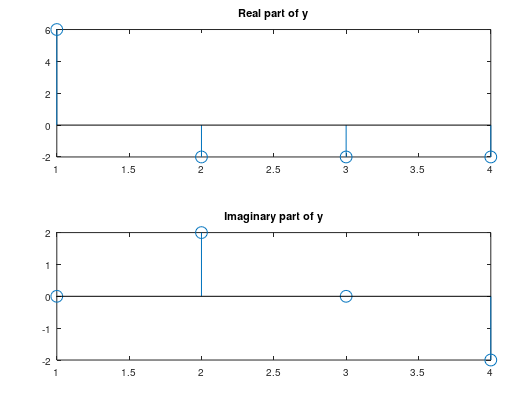
\includegraphics{labss/Lab4_1.PNG}
        \caption{Sample DFT}
    \end{figure}
    \item Sample IDFT: IDFT of Question 1
    \begin{Verbatim}[frame = single]
x = [0,1,2,3]
subplot(4,1,1)
stem(x)
title('x')

y =fft(x)

subplot(4,1,2)
stem(real(y))
title('Real part of y')

subplot(4,1,3)
stem(imag(y))
title('Imaginary part of y')

x = ifft(y)
subplot(4,1,4)
stem(x)
title('Inverse FFT of y')
    \end{Verbatim}
    \begin{figure}[h!]
        \centering
        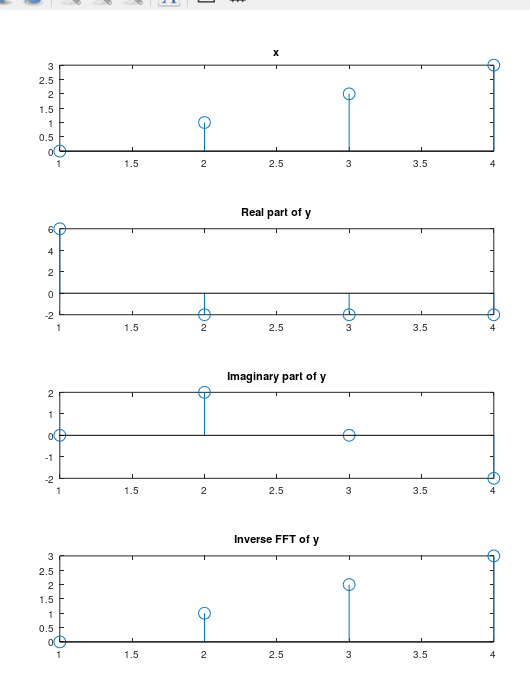
\includegraphics[scale=0.75]{labss/Lab4_2.PNG}
        \caption{Sample IDFT}
    \end{figure}
    \pagebreak
    \item For
    \begin{verbatim}
        x = [1. 2, 3.7, 0.6, 1. 3, 2]
    \end{verbatim}
    \begin{itemize}
        \item Find DFT using FFT.
        \item Find x[n] from the obtained FFT. 
    \end{itemize}
    \begin{Verbatim}[frame = single]
x = [1. 2, 3.7, 0.6, 1. 3, 2]
subplot(4,1,1)
stem(x)
title('x')

y =fft(x)

subplot(4,1,2)
stem(real(y))
title('Real part of y')

subplot(4,1,3)
stem(imag(y))
title('Imaginary part of y')

x = ifft(y)
subplot(4,1,4)
stem(x)
title('Inverse FFT of y')
    \end{Verbatim}
    \begin{figure}[h!]
        \centering
        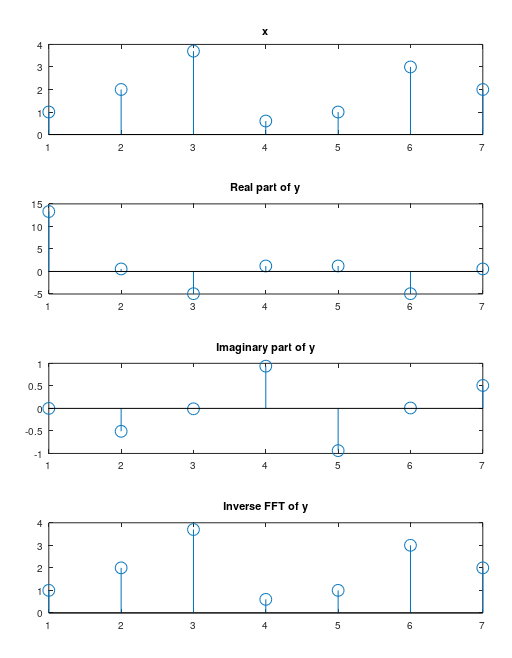
\includegraphics[scale=0.75]{labss/Lab4_3.PNG}
        \caption{FFT and IFFT}
    \end{figure}
    \pagebreak
    \item For
    \begin{equation}
        x = 0.5^n u[n] \nonumber
    \end{equation}
    \begin{itemize}
        \item Find DFT of x[n].
        \item Find x[n] from the obtained FFT. 
    \end{itemize}
    \begin{Verbatim}[frame = single]
x = 0.5 .^t(t>0)
subplot(4,1,1)
stem(x)
title('x')

y =fft(x)

subplot(4,1,2)
stem(real(y))
title('Real part of y')

subplot(4,1,3)
stem(imag(y))
title('Imaginary part of y')

x = ifft(y)
subplot(4,1,4)
stem(x)
title('Inverse FFT of y')

    \end{Verbatim}
    \begin{figure}[h!]
        \centering
        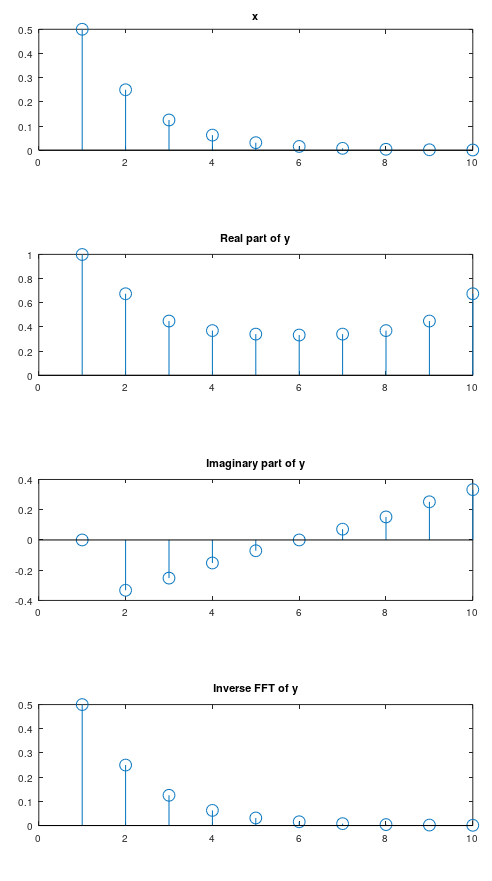
\includegraphics[scale=0.75]{labss/Lab4_4.PNG}
        \caption{FFT and IFFT}
    \end{figure}
\end{enumerate}
\paragraph{Conclusion\\}
In this way "Lab4 : DFT and FFT" was completed through the use of MATLAB. 
\end{document}